%----------------------------------------------------------------------------------------
%	PACKAGES AND OTHER DOCUMENT CONFIGURATIONS
%----------------------------------------------------------------------------------------

\documentclass[paper=a4, fontsize=11pt]{scrartcl} % A4 paper and 11pt font size

\usepackage[T1]{fontenc} % Use 8-bit encoding that has 256 glyphs
\usepackage{fourier} % Use the Adobe Utopia font for the document - comment this line to return to the LaTeX default
\usepackage[english]{babel} % English language/hyphenation
\usepackage{amsmath,amsfonts,amsthm} % Math packages

\usepackage{lipsum} % Used for inserting dummy 'Lorem ipsum' text into the template

\usepackage{sectsty} % Allows customizing section commands
\allsectionsfont{\centering \normalfont\scshape} % Make all sections centered, the default font and small caps
\usepackage{graphicx}
\usepackage{fancyhdr} % Custom headers and footers
\pagestyle{fancyplain} % Makes all pages in the document conform to the custom headers and footers
\fancyhead{} % No page header - if you want one, create it in the same way as the footers below
\fancyfoot[L]{} % Empty left footer
\fancyfoot[C]{} % Empty center footer
\fancyfoot[R]{\thepage} % Page numbering for right footer
\renewcommand{\headrulewidth}{0pt} % Remove header underlines
\renewcommand{\footrulewidth}{0pt} % Remove footer underlines
\setlength{\headheight}{13.6pt} % Customize the height of the header

\numberwithin{equation}{section} 
\numberwithin{figure}{section} 
\numberwithin{table}{section} 

\setlength\parindent{0pt} 

%----------------------------------------------------------------------------------------
%	TITLE SECTION
%----------------------------------------------------------------------------------------

\newcommand{\horrule}[1]{\rule{\linewidth}{#1}}

\title{	
\normalfont \normalsize 
\textsc{Harvard University} \\[25pt]
\textsc{CS281} \\[25pt]
\horrule{0.5pt} \\[0.1cm] 
\huge Final Project Update: \\
\huge Classification for the Yelp Data Set Challenge
\horrule{2pt} \\[0.5cm]
}

\author{Nicolas Drizard \& Virgile Audi}

\date{\normalsize\today} 
\usepackage{float}
\floatplacement{figure}{H} % force figures to be placed always at defined position!

\begin{document}

\maketitle

\section{Data}

We are taking part in the Yelp Dataset challenge round 6. We chosed to solve the question of infering categories based on the reviews. The goal is to build a finer way to categorize the Yelp businesses. The global question is the following: How much information can reviews give us on the type of restaurants?\\

Right now, the users define the label of each entry. This project could be used as an automation tool for Yelp to label properly its data based on the cluster we will find. This would improve the user experience while querying for a specific kind of restaurants.

Data:
\begin{itemize}
		\item 1.6 million reviews
		\item 61 000 businesses
		\item 481 000 attributes (ie hours, parking availabity, take-out, ambience)
		\item aggregated check-in measurements over time
\end{itemize}

We focused first on the restaurants and for one city at a time to grasp in a finer way the local relationships of the restaurants. This also makes more sense on from the user's perspective.\\

\section{Approach}

Our main goal is to build latent features from the text reviews which would depict the categories of the business. To put it in a nutshell, we would like to build from the text reviews of an entry a vector representation which carries local geometry information. Once we built the document-term matrix containing the words count of the reviews for each business (the reviews are aggregated over each restaurant), we could simply use a matrix factorisation on the counts . To be able to interpret the latent features as topics, we could use a Non-negative matrix factorization (the possible negative features in the SVD cannot stand for cluster assignement). A finer result can be reached with the use of a generative probabilistic model, that's why we chosed the latent dirichlet allocation. The LDA uses a Dirichlet prior on the words distribution over the topics and on the topics distribution over the document which will gives them more freedom than the deterministic approach of the NMF.\\

\section{Latent Dirichlet Allocation}

\subsection*{Model}

The LDA is a three-level hierarchical Bayesian model. The basic idea that documents are represented as random mixtures over latent topics and each topic is characterized by a distribution over words.\\

GRAPHICAL MODEL\\


The generation process for a document \textbf{w} in a corpus D is the following:
\begin{enumerate}
	\item Choose the topics representation $\phi \sim$ Dir($\beta$)
	\item Choose the number of words: $ N \sim $ Poisson($ \xi $)
	\item Choose the distribution of topics $\theta_w \sim$ Dir($\alpha_w$)
	\item For each of the N words:
	\begin{enumerate}
		\item Choose a topic assignement $z_{n,w} \sim$ Multinomial($\theta_w$)
		\item Choose a word $w_n \sim$ Multinomial($\phi_{z_{n,w}}$)
	\end{enumerate}
\end{enumerate}

\subsection*{Parameter Estimation}

The main issue relies in computing the posterior distribution of the hidden variables given a document: 
\begin{align*}
p(\theta, \mathbf{z} |\mathbf{w}, \alpha, \beta) = \frac{p(\theta, \mathbf{z}, \mathbf{w} | \alpha, \beta)}{p(\mathbf{w} | \alpha, \beta)}
\end{align*}

This distribution is intractable. There are two main methods to infer it: through a Gibbs sampler or variational inference. In the first case, we are estimating the hyper parameters $\theta$ and $\phi$ with sample on the different variables. The sampling method will converge to the right model is we sample enough but it takes a lot of time. As a result, we chose the variational inference method which find the variational parameters that optimize a lower bound on the log likelihood. To optimize the bound, we use an expectation maximization method where we estimate the topic distribution for the current document based on its word counts in the E-step and then update the topics distribution in the M-step. \\

Moreover, to increase the speed of our algorithm based on the idea that we have enough reviews, we chose the online variational inference method. This enables to go over each data point only once. For comparison, on the reviews from the Las Vegas data set, a gibbs sampler provided by python executed in around 50 minutes whereas our online method executed in less than 1 minute for equivalent topics evaluation.

\subsection*{Evaluation Method}

We need a measure to evaluate the performance of our model and to tune the hyperparameters. We use perplexity on held-out data as a measure of our model fit. Perplexity is defined as the geometric mean of the log likelihood of the words in the held-out set of docuements given the trained model. In our case, for each document we held out 20\% of the words which constitue the test set.

\begin{align*}
	perplexity(D_{test}) & = \frac{\sum_{d \in D_{test}} log p(words)}{\sum_{d \in D_{test}|d|}}\\
	perplexity(D_{test}) & = \frac{\sum_{d \in D_{test}} \sum_{w \in d} log \left( \sum_{t \in topics} p(w|t) * p(t|d) \right)}{\sum_{d \in D_{test}|d|}}
\end{align*}

We used this measure to optimize the number of topics K and the hyper parameters of the optimization of the lower bound.

\subsection*{Next Steps}

So far, we managed to extract the categories of the restaurants as latent features with a latent dirichlet allocation algorithm on the aggregated reviews for each restaurant. \\

A future work could be done on the classification part based on these features: on one hand, clustering the restaurants of different cities and comparing the groups with the existing labels to find new categories or to refine the existing one; on the other hand, we could use the features with classifier to predict the existing categories. \\

As a variant, we could try a supervised LDA, where we use the existing categories as a response variable associated with each document and infer the joint model of the documents and the responses. Lastly, this method is applicable on each review separately to predict the rating of the review, with a supervised lda also to avoid the predominance of the categories in the topics.


\section{Classification}

Once the feature has been extracted, we can apply supervised learning methods to classify the Yelp restaurants based on their labels on Yelp. Several approaches are possible with regards to the features to solve this multi-labels classigication task

\subsection*{Features}

The features are divided into two main parts: on one hand, the topics assignements extracted from the reviews with the LDA and on the other hand, the properties provided by Yelp. Pre-processing the latter part provided a 198 dimensionnal vector. These features contain both numerical features (rating, space coordinates, number of reviews, customer check-in...) and categorical features converted into indicator variables.

\subsection*{Methods}

The outputs of our classification are the labels of each restaurant. We chose to train several binary classifiers to predict one label at a time with a One-Vs-All approach. The high dimensionnality of the features and the large number of indicator varibales induces a high sparsity. As a result, a sufficiently robust algorithm need to be used. One particularity is also that the classes are all really skewed, the dummy baseline where we do not predict  any label for all the restaurant has a really high score.\\

\begin{center}
    \begin{tabular}{| l | l | l | l |}
    \hline
    & OVI LDA & GS LDA & NMF \\ \hline
    All False & 90,02 \% &  90.02 \% &  90.02 \% \\ \hline
    kernel rbf SVM & 90,81\% &  90.38\% &  90.38\% \\ \hline
    kernel rbf SVM + PCA & 90.83\% &  90.60\% &  90.57\% \\ \hline
    Logistic Regression & 90.84\% &  91.89\%  &  91.24\%\\ \hline
    Logistic Regression + PCA & 92.59\% &  92.53\% &  92.68\% \\ \hline
    Lasso & 90.82\% &  93.44\% &  92.01\% \\ \hline
	Lasso + PCA & 93.44\%  &  \textbf{94.46} \%  &  93.08\% \\ \hline
    Random Forest & 91.90\% &  93.31\% &  92.89\% \\ \hline
    Random Forest + PCA & 93.63\% &  94.04\% &  93.44\% \\ \hline
    \end{tabular}
\end{center}

We first coded a l2 regularized logistic regression and use scikit learn for the other methods. The random forest provides the best predictor expected as it corresponds to an ensemble method that combines multiple decision trees, leading to a more robust model. We showed the ROC curves that we obtained. The variance of the classifiers with regards to the class used as output is quite high. This could be explained by the relative skewness of each class and also their own specificity. Moreover, using dimensionality reduction method on the Yelp check-ins information before the classificationthe PCA also improved the accuracy. These features contains the average number of customers for each hour of the week which leads to a vector of dimension 168. The principal component analysis dropped it down to 13, while keeping 94\% of the variance.

\begin{figure}[H]
	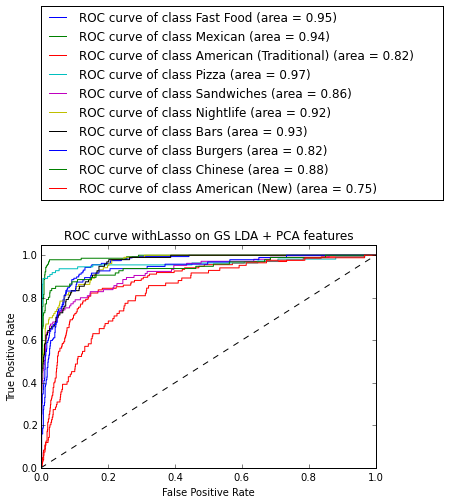
\includegraphics[scale=0.55]{img/roc_lasso.png}
	\centering
\end{figure}

\begin{figure}[H]
	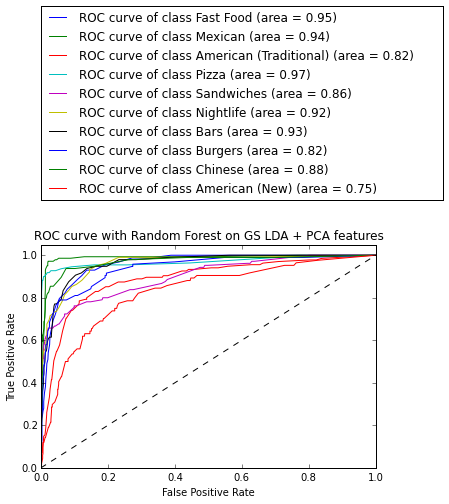
\includegraphics[scale=0.55]{img/roc_rf.png}
	\centering
\end{figure}

Moreover, this method provides a way to sort the features by importance.\\

FEATURES IMPORTANCE





\end{document}